\documentclass[a4paper,11pt]{article}
\usepackage[utf8]{inputenc}
\usepackage[T1]{fontenc}
\usepackage[italian]{babel}
\usepackage{a4wide}
\usepackage{graphicx}
\usepackage[table]{xcolor}
\usepackage{geometry}
\geometry{a4paper,top=2cm,bottom=4cm,left=3cm,right=3cm}
\graphicspath{{../includes/pics/}}

\usepackage{ifthen}
\usepackage{ifpdf}
\ifpdf
\usepackage[pdftex]{hyperref}
\else
\usepackage{hyperref}
\fi
\usepackage{color}
\hypersetup{%
colorlinks=true,
linkcolor=black,
citecolor=black,
urlcolor=blue}
\usepackage[nonumberlist,section=subsection]{glossaries}
\usepackage{lastpage}
\usepackage{afterpage}
\setcounter{secnumdepth}{5}
\setcounter{tocdepth}{5}
\usepackage{subfig}
\usepackage{rotating}
\usepackage{pdflscape}
\usepackage{tikz}
\usepackage{ragged2e}
\usepackage{tabularx}
\usepackage{longtable}
\usetikzlibrary{shapes,arrows}
\usepackage{pgfplots}
\pgfplotsset{compat=newest}
\pgfplotsset{plot coordinates/math parser=false}

\usepackage{fancyhdr}
\usepackage{eurosym}
\usepackage{colortbl}
\usepackage{float}
\usepackage{amsthm}
\usepackage{amssymb,amsmath}
\usepackage{array}
\usepackage{bm}
\usepackage{multirow}
\usepackage[footnote]{acronym}
\usepackage[bottom]{footmisc}
%%%%%%%%%%%%%%%%%%%%%%%%%%%%%%%%%%%%%%%%%%%%%%%%%%%%%%%%%%%%%%%%%%%%%
% COMANDI DA RIDEFINIRE
%%%%%%%%%%%%%%%%%%%%%%%%%%%%%%%%%%%%%%%%%%%%%%%%%%%%%%%%%%%%%%%%%%%%%

%TITOLO
%%%%%%%%%%%%%%%%%%%%%%%%%%%%%%%%%%%%%%%%%%%%%%%%%%%%%%%%%%%%%%%%%%%%%
\newcommand{\thetitle}{TEMPLATE}
%%%%%%%%%%%%%%%%%%%%%%%%%%%%%%%%%%%%%%%%%%%%%%%%%%%%%%%%%%%%%%%%%%%%%

%VERSIONE
%%%%%%%%%%%%%%%%%%%%%%%%%%%%%%%%%%%%%%%%%%%%%%%%%%%%%%%%%%%%%%%%%%%%%
\newcommand{\theversion}{ 0.0.0 }
%%%%%%%%%%%%%%%%%%%%%%%%%%%%%%%%%%%%%%%%%%%%%%%%%%%%%%%%%%%%%%%%%%%%%

%DATA
%%%%%%%%%%%%%%%%%%%%%%%%%%%%%%%%%%%%%%%%%%%%%%%%%%%%%%%%%%%%%%%%%%%%%
\newcommand{\thedate}{ 00 Mese 2018 }
%%%%%%%%%%%%%%%%%%%%%%%%%%%%%%%%%%%%%%%%%%%%%%%%%%%%%%%%%%%%%%%%%%%%%

%DATA (Ultima modifica)
%%%%%%%%%%%%%%%%%%%%%%%%%%%%%%%%%%%%%%%%%%%%%%%%%%%%%%%%%%%%%%%%%%%%%
\newcommand{\thedatelast}{ 00 Mese 2018 }
%%%%%%%%%%%%%%%%%%%%%%%%%%%%%%%%%%%%%%%%%%%%%%%%%%%%%%%%%%%%%%%%%%%%%

%USO (INTERNO/ESTERNO)
%%%%%%%%%%%%%%%%%%%%%%%%%%%%%%%%%%%%%%%%%%%%%%%%%%%%%%%%%%%%%%%%%%%%%
\newcommand{\usage}{ Interno/Esterno }
%%%%%%%%%%%%%%%%%%%%%%%%%%%%%%%%%%%%%%%%%%%%%%%%%%%%%%%%%%%%%%%%%%%%%

%STATO
%%%%%%%%%%%%%%%%%%%%%%%%%%%%%%%%%%%%%%%%%%%%%%%%%%%%%%%%%%%%%%%%%%%%%
\newcommand{\status}{ Da Approvare/Approvato/.. }
%%%%%%%%%%%%%%%%%%%%%%%%%%%%%%%%%%%%%%%%%%%%%%%%%%%%%%%%%%%%%%%%%%%%%

%RESPONSABILE
%%%%%%%%%%%%%%%%%%%%%%%%%%%%%%%%%%%%%%%%%%%%%%%%%%%%%%%%%%%%%%%%%%%%%
\newcommand{\resp}{Unico Responsabile}
%%%%%%%%%%%%%%%%%%%%%%%%%%%%%%%%%%%%%%%%%%%%%%%%%%%%%%%%%%%%%%%%%%%%%

%VERIFICATORI
%%%%%%%%%%%%%%%%%%%%%%%%%%%%%%%%%%%%%%%%%%%%%%%%%%%%%%%%%%%%%%%%%%%%%
\newcommand{\verif}{Primo Verificatore, Secondo Verificatore}
%%%%%%%%%%%%%%%%%%%%%%%%%%%%%%%%%%%%%%%%%%%%%%%%%%%%%%%%%%%%%%%%%%%%%

%REDAZIONE
%%%%%%%%%%%%%%%%%%%%%%%%%%%%%%%%%%%%%%%%%%%%%%%%%%%%%%%%%%%%%%%%%%%%%
\newcommand{\editorfrow}{Membri Redazione, Prima Riga}
\newcommand{\editorsrow}{Membri Redazione, Seconda Riga}
%%%%%%%%%%%%%%%%%%%%%%%%%%%%%%%%%%%%%%%%%%%%%%%%%%%%%%%%%%%%%%%%%%%%%

%NOME PROPONENTE
%%%%%%%%%%%%%%%%%%%%%%%%%%%%%%%%%%%%%%%%%%%%%%%%%%%%%%%%%%%%%%%%%%%%%
\newcommand{\proposer}{zero12}
%%%%%%%%%%%%%%%%%%%%%%%%%%%%%%%%%%%%%%%%%%%%%%%%%%%%%%%%%%%%%%%%%%%%%

%DESCRIZIONE
%%%%%%%%%%%%%%%%%%%%%%%%%%%%%%%%%%%%%%%%%%%%%%%%%%%%%%%%%%%%%%%%%%%%%
\newcommand{\descript}{
	\\[0.65cm]
	\textbf{Descrizione}\\
	Documento esterno, disponibile per la visione alla proponente \emph{Zero12}, \\che delinea le funzionalità del prodotto realizzate dal Gruppo \emph{duckware}.
	\\[0.65cm]	
}
%%%%%%%%%%%%%%%%%%%%%%%%%%%%%%%%%%%%%%%%%%%%%%%%%%%%%%%%%%%%%%%%%%%%%

%CONTENUTI
%%%%%%%%%%%%%%%%%%%%%%%%%%%%%%%%%%%%%%%%%%%%%%%%%%%%%%%%%%%%%%%%%%%%%
\newcommand{\contents}{
	\section{Introduzione}
\addcontentsline{toc}{section}{Introduzione}
\markboth{Introduction}{Introduzione}
\label{sec:introduzione}
%\minitoc

Lorem ipsum dolor sit amet, consectetur adipiscing elit. Sed non risus. Suspendisse lectus tortor, dignissim sit amet, adipiscing nec, ultricies sed, dolor. Cras elementum ultrices diam. Maecenas ligula massa, varius a, semper congue, euismod non, mi. Proin porttitor, orci nec nonummy molestie, enim est eleifend mi, non fermentum diam nisl sit amet erat. Duis semper. Duis arcu massa, scelerisque vitae, consequat in, pretium a, enim.

\section{Casi d'Uso}
\label{sec:casiduso}

\subsection{Una Sottosezioneee}
Lorem ipsum dolor sit amet, consectetur adipiscing elit \cite{Roque2012,Roque2012b,Roque2012c,Roque2012d}. Sed non risus. Suspendisse lectus tortor, dignissim sit amet, adipiscing nec, ultricies sed, dolor. Cras elementum ultrices diam. Maecenas ligula massa, varius a, semper congue, euismod non, mi. Proin porttitor, orci nec nonummy molestie, enim est eleifend mi, non fermentum diam nisl sit amet erat. Duis semper. Duis arcu massa, scelerisque vitae, consequat in, pretium a, enim. Pellentesque congue. Ut in risus volutpat libero pharetra tempor. Cras vestibulum bibendum augue. Praesent egestas leo in pede. Praesent blandit odio eu enim. Pellentesque sed dui ut augue blandit sodales. Vestibulum ante ipsum primis in faucibus orci luctus et ultrices posuere cubilia Curae; Aliquam nibh. Mauris ac mauris sed pede pellentesque fermentum. Curabitur eu amet (fig. \ref{fig:une-image}). Deux citations \cite{Arapoglou2011,Roque2013c}.

%\begin{figure}[htp]
%  \centering
%  \input{images/tikz_diagram} %inserisce diagramma
%  \caption{Esempio di diagramma TikZ.} %inserisce didascalia
%  \label{fig:una-immagine}
%\end{figure}

\begin{table}[ht]
  \begin{center}
	\rowcolors{1}{white}{lightgray}   %COLORE RIGHE DELLA TABELLA: PARTENDO DA RIGA 1 -> DISPARI BIANCO, PARI GRIGIO
	\begin{tabularx}{\linewidth}{
    	|>{\hsize=.3\hsize}X|% 
    	>{\hsize=.7\hsize}X|%
    	>{\hsize=.65\hsize}X|% 
    	>{\hsize=.95\hsize}X|%
    	>{\hsize=2.4\hsize}X|%
       % sum=5.0\hsize for 5 columns
  	}
    	\hline
    	\textbf{Ver.}&\textbf{Data}&\textbf{Autore}&\textbf{Ruolo}&\textbf{Descrizione}\\
    	\hline
    	x.x.x & 2018/12/01 & Alessandro Pegoraro & Amministratore & Lorem ipsum dolor sit amet, consectetur adipiscing elit.\\
    	\hline
    \end{tabularx}
    \caption{Esempio di Tabella}
    \label{tab:unatabella}
  \end{center}
\end{table}

%\begin{figure}[htp]
%  \centering
%  \includegraphics[width=4cm]{images/bitmap_image} %inserisce immagine
%  \caption{Esempio di immagine JPG.}
%  \label{fig:un-altra-immagine}
%\end{figure}

\section{Tecnologie}
\label{sec:tecnologie}

Lorem ipsum dolor sit amet, consectetur adipiscing elit. Sed non risus. Suspendisse lectus tortor, dignissim sit amet, adipiscing nec, ultricies sed, dolor. Cras elementum ultrices diam. Maecenas ligula massa, varius a, semper congue, euismod non, mi. Proin porttitor, orci nec nonummy molestie, enim est eleifend mi, non fermentum diam nisl sit amet erat. Duis semper. Duis arcu massa, scelerisque vitae,  convallis sollicitudin purus. Praesent aliquam, enim at fermentum mollis, ligula massa adipiscing nisl, ac euismod nibh nisl eu lectus. Fusce vulputate sem at sapien. Vivamus leo. Aliquam euismod libero eu enim. Nulla nec felis sed leo placerat imperdiet. Aenean suscipit nulla in justo. Suspendisse cursus rutrum augue. Nulla tincidunt tincidunt mi. Curabitur iaculis, lorem vel rhoncus faucibus, felis magna fermentum augue, et ultricies lacus lorem varius purus. Curabitur eu amet. Encore une citation \cite{Cadambe2008}.


\section*{Conclusioni}
\addcontentsline{toc}{section}{Conclusioni}
\markboth{Conclusioni}{Conclusioni}
\label{sec:conclusioni}
Lorem ipsum dolor sit amet, consectetur adipiscing elit. Sed non risus. Suspendisse lectus tortor, dignissim sit amet, adipiscing nec, ultricies sed, dolor. Cras elementum ultrices diam. Maecenas ligula massa, varius a, semper congue, euismod non, mi. Proin porttitor, orci nec nonummy molestie, enim est eleifend mi, non fermentum diam nisl sit amet erat. Duis semper. Duis arcu massa, scelerisque vitae, consequat in, pretium a, enim. Pellentesque congue. Ut in risus volutpat libero pharetra tempor. Cras vestibulum bibendum augue. Praesent egestas leo in pede. Praesent blandit odio eu enim.

\clearpage
}
%%%%%%%%%%%%%%%%%%%%%%%%%%%%%%%%%%%%%%%%%%%%%%%%%%%%%%%%%%%%%%%%%%%%%

%%%%%%%%%%%%%%%%%%%%%%%%%%%%%%%%%%%%%%%%%%%%%%%%%%%%%%%%%%%%%%%%%%%%%
% COMANDI DA NON RIDEFINIRE
%%%%%%%%%%%%%%%%%%%%%%%%%%%%%%%%%%%%%%%%%%%%%%%%%%%%%%%%%%%%%%%%%%%%%

%NOME E EMAIL GRUPPO
%%%%%%%%%%%%%%%%%%%%%%%%%%%%%%%%%%%%%%%%%%%%%%%%%%%%%%%%%%%%%%%%%%%%%
\newcommand{\groupName}{duckware}
\newcommand{\groupEmail}{duckware.swe@gmail.com}
%%%%%%%%%%%%%%%%%%%%%%%%%%%%%%%%%%%%%%%%%%%%%%%%%%%%%%%%%%%%%%%%%%%%%

%NOME MEMBRI DEL GRUPPO
%%%%%%%%%%%%%%%%%%%%%%%%%%%%%%%%%%%%%%%%%%%%%%%%%%%%%%%%%%%%%%%%%%%%%
\newcommand{\luca}{\mbox{Luca} \textsc{\mbox{Stocco}}}
\newcommand{\sonia}{\mbox{Sonia} \textsc{\mbox{Menon}}}
\newcommand{\alberto}{\mbox{Alberto} \textsc{\mbox{Miola}}}
\newcommand{\pardeep}{\mbox{Pardeep} \textsc{\mbox{Singh}}}
\newcommand{\matteo}{\mbox{Matteo} \textsc{\mbox{Pellanda}}}
\newcommand{\alessandro}{\mbox{Alessandro} \textsc{\mbox{Pegoraro}}}
\newcommand{\andrea}{\mbox{Andrea} \textsc{\mbox{Pavin}}}
%%%%%%%%%%%%%%%%%%%%%%%%%%%%%%%%%%%%%%%%%%%%%%%%%%%%%%%%%%%%%%%%%%%%%

%NOME DEI DOCUMENTI
%%%%%%%%%%%%%%%%%%%%%%%%%%%%%%%%%%%%%%%%%%%%%%%%%%%%%%%%%%%%%%%%%%%%%
\newcommand{\SdF}{Studio di Fattibilità}
\newcommand{\PdP}{Piano di Progetto}
\newcommand{\PdQ}{Piano di Qualifica}
\newcommand{\AdR}{Analisi dei Requisiti}
\newcommand{\NdP}{Norme di Progetto}
\newcommand{\Glos}{Glossario}
\newcommand{\Ver}{Verbale}
%%%%%%%%%%%%%%%%%%%%%%%%%%%%%%%%%%%%%%%%%%%%%%%%%%%%%%%%%%%%%%%%%%%%%

%ATTIVITA' DEL CHANGELOG
%%%%%%%%%%%%%%%%%%%%%%%%%%%%%%%%%%%%%%%%%%%%%%%%%%%%%%%%%%%%%%%%%%%%%
\newcommand{\creazione}{Creazione scheletro del documento}
\newcommand{\stesura}[1]{Stesura #1}
\newcommand{\rimozione}[1]{Rimozione #1}
\newcommand{\inserimento}[1]{Inserimento #1}
\newcommand{\modifica}[1]{Modifica #1}
\newcommand{\correzione}[1]{Correzione #1}
\newcommand{\verifica}[1]{Superamento verifica #1}
\newcommand{\approvazione}[1]{Approvazione per rilascio del documento in #1}
\newcommand{\analisi}[1]{Analisi e stesura #1}
\newcommand{\update}{Aggiornamento del documento}

%COMANDO PER AGGIUNGERE IL RIFERIMENTO AL PARAGRAFO (#1 = NOME DELLA LABEL)
\newcommand{\addref}[1]{\hyperref[#1]{\textsection \ref*{#1}}}
%%%%%%%%%%%%%%%%%%%%%%%%%%%%%%%%%%%%%%%%%%%%%%%%%%%%%%%%%%%%%%%%%%%%%

%COLORI TABELLE
%%%%%%%%%%%%%%%%%%%%%%%%%%%%%%%%%%%%%%%%%%%%%%%%%%%%%%%%%%%%%%%%%%%%%
\definecolor{tableHeadYellow}{rgb}{1.0, 0.88, 0.21}
\definecolor{tableLightYellow}{rgb}{1.0, 0.97, 0.86}
%%%%%%%%%%%%%%%%%%%%%%%%%%%%%%%%%%%%%%%%%%%%%%%%%%%%%%%%%%%%%%%%%%%%%

%NUMERAZIONE PAGINE
%%%%%%%%%%%%%%%%%%%%%%%%%%%%%%%%%%%%%%%%%%%%%%%%%%%%%%%%%%%%%%%%%%%%%
\newcommand{\cambiastile}{\fancyfoot[R]{Pagina \thepage{} di \pageref{LastPage}}}
%%%%%%%%%%%%%%%%%%%%%%%%%%%%%%%%%%%%%%%%%%%%%%%%%%%%%%%%%%%%%%%%%%%%%

%%%%%%%%%%%%%%%%%%%%%%%%%%%%%%%%%%%%%%%%%%%%%%%%%%%%%%%%%%%%%%%%%%%%%
% UTILITIES
%%%%%%%%%%%%%%%%%%%%%%%%%%%%%%%%%%%%%%%%%%%%%%%%%%%%%%%%%%%%%%%%%%%%%

%Inserisce Pagina Bianca
%%%%%%%%%%%%%%%%%%%%%%%%%%%%%%%%%%%%%%%%%%%%%%%%%%%%%%%%%%%%%%%%%%%%%
\newcommand\blankpage{%
    \null
    \newpage}
%%%%%%%%%%%%%%%%%%%%%%%%%%%%%%%%%%%%%%%%%%%%%%%%%%%%%%%%%%%%%%%%%%%%

%Impostazioni Glossario
%%%%%%%%%%%%%%%%%%%%%%%%%%%%%%%%%%%%%%%%%%%%%%%%%%%%%%%%%%%%%%%%%%%%%

\newcommand{\markg}[1]{\textit{#1}\textsubscript{\textit{G}}} %MACRO PER INSERIRE "G" A PEDICE
\makeglossaries
\loadglsentries{../../../../Template_Latex/glsentries} %CARICA LE ENTRIES DEL GLOSSARIO
\newglossarystyle{dict}%
{%
  \renewcommand*{\glossaryheader}{}%
  \renewcommand*{\glsgroupheading}[1]{%
 	 \ifstrequal{A}{##1}{}%
	{\clearpage}%  
    \section*{##1}% 
    \addcontentsline{toc}{section}{##1} 
  }%
  \renewcommand{\glossaryentryfield}[5]{%
    \markboth{##2}{##2}%
    \par\vspace{0.25\baselineskip}%
    \textbf{\textsf{##2}} \textit{- ##4 -} ##3%
  }%
}%

%%%%%%%%%%%%%%%%%%%%%%%%%%%%%%%%%%%%%%%%%%%%%%%%%%%%%%%%%%%%%%%%%%%%%
\newlength\figureheight
\newlength\figurewidth
\pgfkeys{/pgf/number format/.cd,
set decimal separator={,\!},
1000 sep={\,},
}
\renewcommand{\baselinestretch}{1.05}

%FANCYPAGESTYLE
%%%%%%%%%%%%%%%%%%%%%%%%%%%%%%%%%%%%%%%%%%%%%%%%%%%%%%%%%%%%%%%%%%%%%
\pagestyle{fancy}
\fancyfoot[R]{\thepage}
\fancyfoot[L]{\thetitle}
\fancyfoot[C]{}
\fancyhead[R]{
\includegraphics[width=0.15\textwidth]{../../../../Template_Latex/logo}}
\fancyhead[L]{\bfseries\nouppercase{\leftmark}}
\setlength{\headheight}{30pt}
%%%%%%%%%%%%%%%%%%%%%%%%%%%%%%%%%%%%%%%%%%%%%%%%%%%%%%%%%%%%%%%%%%%%%

\let\headruleORIG\headrule
\renewcommand{\headrule}{\color{black} \headruleORIG}
\renewcommand{\headrulewidth}{1.0pt}

\arrayrulecolor{black}

\let\footruleORIG\footrule
\renewcommand{\footrule}{\color{black} \footruleORIG}
\renewcommand{\footrulewidth}{1.0pt}

\fancypagestyle{plain}{
  \fancyhead{}
  \fancyfoot[C]{\thepage}
  \renewcommand{\headrulewidth}{0pt}
  \renewcommand{\footrulewidth}{0pt}
}

\parskip=5pt

\begin{document}
	%RIDEFINIZIONE COMANDI
	%%%%%%%%%%%%%%%%%%%%%%%%%%%%%%%%%%%%%%%%%%%%%%%%%%%%%%%%%%%%%%%%%%%%%
	\renewcommand{\thetitle}{ Piano di Qualifica }
	\renewcommand{\thedate}{ 04 Gennaio 2019 }
	\renewcommand{\theversion}{ 1.0.0 }
	%%%%%%%%%%%%%%%%%%%%%%%%%%%%%%%%%%%%%%%%%%%%%%%%%%%%%%%%%%%%%%%%%%%%%
	
	%COMANDI PER PRIMA PAGINA
	%%%%%%%%%%%%%%%%%%%%%%%%%%%%%%%%%%%%%%%%%%%%%%%%%%%%%%%%%%%%%%%%%%%%%
	\renewcommand{\usage}{Esterno}
	\renewcommand{\status}{Approvato}
	\renewcommand{\verif}{\andrea , \alberto}
	\renewcommand{\resp}{\matteo}
	\renewcommand{\editorfrow}{\luca , \sonia}
	\renewcommand{\editorsrow}{\alessandro , \pardeep}
	\renewcommand{\proposer}{zero12}
	%%%%%%%%%%%%%%%%%%%%%%%%%%%%%%%%%%%%%%%%%%%%%%%%%%%%%%%%%%%%%%%%%%%%%
	
	%CONTENUTI
	%%%%%%%%%%%%%%%%%%%%%%%%%%%%%%%%%%%%%%%%%%%%%%%%%%%%%%%%%%%%%%%%%%%%%
	\renewcommand{\contents}{
		\section{Introduzione}
\addcontentsline{toc}{section}{Introduzione}
\markboth{Introduction}{Introduzione}
\label{sec:introduzione}
%\minitoc

Lorem ipsum dolor sit amet, consectetur adipiscing elit. Sed non risus. Suspendisse lectus tortor, dignissim sit amet, adipiscing nec, ultricies sed, dolor. Cras elementum ultrices diam. Maecenas ligula massa, varius a, semper congue, euismod non, mi. Proin porttitor, orci nec nonummy molestie, enim est eleifend mi, non fermentum diam nisl sit amet erat. Duis semper. Duis arcu massa, scelerisque vitae, consequat in, pretium a, enim.

\section{Casi d'Uso}
\label{sec:casiduso}

\subsection{Una Sottosezioneee}
Lorem ipsum dolor sit amet, consectetur adipiscing elit \cite{Roque2012,Roque2012b,Roque2012c,Roque2012d}. Sed non risus. Suspendisse lectus tortor, dignissim sit amet, adipiscing nec, ultricies sed, dolor. Cras elementum ultrices diam. Maecenas ligula massa, varius a, semper congue, euismod non, mi. Proin porttitor, orci nec nonummy molestie, enim est eleifend mi, non fermentum diam nisl sit amet erat. Duis semper. Duis arcu massa, scelerisque vitae, consequat in, pretium a, enim. Pellentesque congue. Ut in risus volutpat libero pharetra tempor. Cras vestibulum bibendum augue. Praesent egestas leo in pede. Praesent blandit odio eu enim. Pellentesque sed dui ut augue blandit sodales. Vestibulum ante ipsum primis in faucibus orci luctus et ultrices posuere cubilia Curae; Aliquam nibh. Mauris ac mauris sed pede pellentesque fermentum. Curabitur eu amet (fig. \ref{fig:une-image}). Deux citations \cite{Arapoglou2011,Roque2013c}.

%\begin{figure}[htp]
%  \centering
%  \input{images/tikz_diagram} %inserisce diagramma
%  \caption{Esempio di diagramma TikZ.} %inserisce didascalia
%  \label{fig:una-immagine}
%\end{figure}

\begin{table}[ht]
  \begin{center}
	\rowcolors{1}{white}{lightgray}   %COLORE RIGHE DELLA TABELLA: PARTENDO DA RIGA 1 -> DISPARI BIANCO, PARI GRIGIO
	\begin{tabularx}{\linewidth}{
    	|>{\hsize=.3\hsize}X|% 
    	>{\hsize=.7\hsize}X|%
    	>{\hsize=.65\hsize}X|% 
    	>{\hsize=.95\hsize}X|%
    	>{\hsize=2.4\hsize}X|%
       % sum=5.0\hsize for 5 columns
  	}
    	\hline
    	\textbf{Ver.}&\textbf{Data}&\textbf{Autore}&\textbf{Ruolo}&\textbf{Descrizione}\\
    	\hline
    	x.x.x & 2018/12/01 & Alessandro Pegoraro & Amministratore & Lorem ipsum dolor sit amet, consectetur adipiscing elit.\\
    	\hline
    \end{tabularx}
    \caption{Esempio di Tabella}
    \label{tab:unatabella}
  \end{center}
\end{table}

%\begin{figure}[htp]
%  \centering
%  \includegraphics[width=4cm]{images/bitmap_image} %inserisce immagine
%  \caption{Esempio di immagine JPG.}
%  \label{fig:un-altra-immagine}
%\end{figure}

\section{Tecnologie}
\label{sec:tecnologie}

Lorem ipsum dolor sit amet, consectetur adipiscing elit. Sed non risus. Suspendisse lectus tortor, dignissim sit amet, adipiscing nec, ultricies sed, dolor. Cras elementum ultrices diam. Maecenas ligula massa, varius a, semper congue, euismod non, mi. Proin porttitor, orci nec nonummy molestie, enim est eleifend mi, non fermentum diam nisl sit amet erat. Duis semper. Duis arcu massa, scelerisque vitae,  convallis sollicitudin purus. Praesent aliquam, enim at fermentum mollis, ligula massa adipiscing nisl, ac euismod nibh nisl eu lectus. Fusce vulputate sem at sapien. Vivamus leo. Aliquam euismod libero eu enim. Nulla nec felis sed leo placerat imperdiet. Aenean suscipit nulla in justo. Suspendisse cursus rutrum augue. Nulla tincidunt tincidunt mi. Curabitur iaculis, lorem vel rhoncus faucibus, felis magna fermentum augue, et ultricies lacus lorem varius purus. Curabitur eu amet. Encore une citation \cite{Cadambe2008}.


\section*{Conclusioni}
\addcontentsline{toc}{section}{Conclusioni}
\markboth{Conclusioni}{Conclusioni}
\label{sec:conclusioni}
Lorem ipsum dolor sit amet, consectetur adipiscing elit. Sed non risus. Suspendisse lectus tortor, dignissim sit amet, adipiscing nec, ultricies sed, dolor. Cras elementum ultrices diam. Maecenas ligula massa, varius a, semper congue, euismod non, mi. Proin porttitor, orci nec nonummy molestie, enim est eleifend mi, non fermentum diam nisl sit amet erat. Duis semper. Duis arcu massa, scelerisque vitae, consequat in, pretium a, enim. Pellentesque congue. Ut in risus volutpat libero pharetra tempor. Cras vestibulum bibendum augue. Praesent egestas leo in pede. Praesent blandit odio eu enim.

\clearpage
	}
	%%%%%%%%%%%%%%%%%%%%%%%%%%%%%%%%%%%%%%%%%%%%%%%%%%%%%%%%%%%%%%%%%%%%%

	%PRIMA PAGINA
	%%%%%%%%%%%%%%%%%%%%%%%%%%%%%%%%%%%%%%%%%%%%%%%%%%%%%%%%%%%%%%%%%%%%%
	%PRIMA PAGINA
%%%%%%%%%%%%%%%%%%%%%%%%%%%%%%%%%%%%%%%%%%%%%%%%%%%%%%%%%%%%%%%%%%%%%
\begin{titlepage}
\begin{center}

\includegraphics[width=0.5\textwidth]{../../../../Template_Latex/logo}\\
{\large INGEGNERIA DEL SOFTWARE \\ a.a. 2018/2019}\\[0.5cm]
{\large Capitolato C4 - MegAlexa}\\
\rule{\linewidth}{0.5mm} \\[0.4cm]
{ \huge \bfseries \thetitle \\[0.4cm] } %TITOLO
\rule{\linewidth}{0.5mm} \\[1.cm]
\noindent
\begin{minipage}{0.4\textwidth}
	\begin{flushleft} \large
		\underline{\emph{Componenti:}}\\[0.2cm]
		\sonia\\
		\alberto \\
		\andrea  \\
		\alessandro \\
		\matteo  \\ 
		\pardeep \\  
		\luca \\
	\end{flushleft}
\end{minipage}
\begin{minipage}{0.4\textwidth}
  \begin{flushright} \large
    \underline{\emph{Destinatari:}} \\[0.2cm]
    Prof.~Tullio \textsc{Vardanega}\\
    Prof.\hspace{0.31cm}~Riccardo \textsc{Cardin}\\
    \proposer
  \end{flushright}
\end{minipage}\\[0.8cm]

\underline{\emph{Informazioni sul documento}} \\[0.2cm]
\begin{tabular}{ll}
	\emph{Responsabile} & \resp \\
	\emph{Verifica} & \verif \\
	\emph{Redazione} & \editorfrow \\
					 & \editorsrow \\  
	\emph{Uso} & \usage\\
	\emph{Stato} & \status\\
	\emph{Email} & \href{mailto:\groupEmail} {\groupEmail}\\
	\emph{Riferimento} & \href{https://www.math.unipd.it/~tullio/IS-1/2018/Progetto/C4.pdf}{Capitolato C4 - MegAlexa}
\end{tabular}
	\descript %INSERISCE DESCRIZIONE DI desc_documento.tex 
\vfill
{\large Versione \theversion{} del\\ \thedate} %BOTTOM
\end{center}
\end{titlepage}
%%%%%%%%%%%%%%%%%%%%%%%%%%%%%%%%%%%%%%%%%%%%%%%%%%%%%%%%%%%%%%%%%%%%%
	%%%%%%%%%%%%%%%%%%%%%%%%%%%%%%%%%%%%%%%%%%%%%%%%%%%%%%%%%%%%%%%%%%%%%

	%INDICE E CHANGELOG
	%%%%%%%%%%%%%%%%%%%%%%%%%%%%%%%%%%%%%%%%%%%%%%%%%%%%%%%%%%%%%%%%%%%%%
	\pagenumbering{roman} %enumerazione pagine per indice
	\tableofcontents %crea indice
	\pagebreak 
	\listoftables	
	\pagebreak  %toglie pagina vuota in più
	\pagenumbering{gobble} %esclude dalla numerazione 
	\section*{Registro delle modifiche}
\addcontentsline{toc}{section}{Registro delle modifiche}
\begin{center}
	\renewcommand{\arraystretch}{1.5}
	\rowcolors{3}{tableLightYellow}{}
	\begin{longtable}{  >{\RaggedRight}p{.8cm}  >{\RaggedRight}p{1.8cm} >{\RaggedRight}p{1.8cm} >{\RaggedRight}p{2.5cm} >{\RaggedRight}p{6cm} }
    	\rowcolor{tableHeadYellow}
    	\textbf{Ver.}&\textbf{Data}&\textbf{Autore}&\textbf{Ruolo}&\textbf{Descrizione}\\
    		
    		%3.0.4 & 2019-05-03 & \matteo & Verificatore & \correzione{\addref{sec:copertura_req}}\\
    		
    		3.0.4 & 2019-05-03 & \matteo & Verificatore & \correzione{\addref{sec:copertura_req}}\\
    		
    		3.0.3 & 2019-05-02 & \matteo & Verificatore & \correzione{codici metriche in \addref{sec:revisione_progettazione}, \addref{sec:revisione_qualifica} e \addref{sec:revisione_accettazione}}\\
    		
    		3.0.2 & 2019-04-29 & \alberto & Verificatore & \verifica{notifica di errore codici metriche in \addref{sec:revisione_progettazione}, \addref{sec:revisione_qualifica} e \addref{sec:revisione_accettazione}}\\
    	 	3.0.1 & 2019-04-28 & \matteo & Redattore & \stesura{\addref{sec:revisione_accettazione}}\\
    	    3.0.0 & 2019-04-09 & \alessandro & Responsabile & \approvazione{RQ}\\
    	    2.0.5 & 2019-04-09 & \alberto & Verificatore & \verifica{ \addref{sec:revisione_qualifica}}\\
    		2.0.4 & 2019-04-08 & \matteo & Redattore & Aggiunti grafici in{ \addref{sec:revisione_qualifica}}\\
    		2.0.3 & 2019-04-07 & \matteo & Redattore & Piccole modifiche in{ \addref{sec:revisione_qualifica}}\\
    		2.0.2 & 2019-04-02 & \matteo & Redattore & \stesura{\addref{sec:revisione_qualifica}}\\
    		2.0.1 & 2019-03-23 & \pardeep & Redattore & Piccole modifiche in{ \addref{sec:ref}}\\
    		2.0.0 & 2019-03-07 & \matteo & Responsabile & \approvazione{RP}\\
    		1.1.0 & 2019-03-07 & \andrea & Verificatore & \verifica{documento}\\
    	    1.0.10 & 2019-03-06 & \pardeep & Amministratore & Aggiornamento e modifiche alle metriche in \addref{sec:qualita_processo}\\
    	    1.0.9 & 2019-03-05 & \andrea & Amministratore & \update{ resoconto \addref{sec:revisione_progettazione}}\\
    		1.0.8 & 2019-03-05 & \matteo & Amministratore & Inserimento resoconto in \addref{sec:revisione_progettazione}\\
    		1.0.7 & 2019-03-01 & \matteo & Amministratore & Inserimento metriche di qualità dei processi in \addref{sec:qualita_processo}\\
    		1.0.6 & 2019-03-01 & \matteo & Amministratore & Alcune correzzioni in 
    		\addref{sec:qualita_prodotto} e \addref{sec:qualita_processo}\\
    		1.0.5 & 2019-02-24 & \matteo & Amministratore & \rimozione{\textit{"Specifiche dei test"}}\\
    		1.0.4 & 2019-02-18 & \matteo & Amministratore & \correzione{dei riferimenti in \addref{sec:ref} e aggiunte al footnote}\\
    		1.0.3 & 2019-02-17 & \pardeep & Amministratore & \modifica{in \addref{sec:qualita_prodotto}: suddivisione in paragrafo su qualità dei documenti
    		 \addref{sec:qualita_documenti} e qualità software \addref{sec:qualita_software_parag}}\\
    		1.0.2 & 2019-02-17 & \matteo & Amministratore & \correzione{dei titoli secondo valutazione RR} \\
    	    1.0.1 & 2019-02-15 & \alberto & Verificatore & \correzione{errori di sintassi e di contenuto}\\
			1.0.0 & 2019-01-04 & \matteo & Responsabile & \approvazione{RR}\\
			0.1.7 & 2019-01-04 & \andrea & Verificatore &  \verifica{completa}\\
			0.1.6 & 2019-01-02 & \andrea & Verificatore &  \correzione{errori in \addref{sec:qualita_software}}\\
			0.1.5 & 2019-01-01 & \alberto & Verificatore & \correzione{errori in \addref{sec:resoconto}}\\
			0.1.4 & 2018-12-31 & \alessandro & Amministratore & \modifica{\addref{sec:resoconto}}\\
			0.1.3 & 2018-12-29 & \sonia & Amministratore & \rimozione{\textit{"Misure e metriche"}}\\
			0.1.2 & 2018-12-26 & \sonia & Amministratore & \stesura{\addref{sec:resoconto}}\\
			0.1.1 & 2018-12-09 & \pardeep & Amministratore & \stesura{\textit{"Misure e metriche"}}\\
			0.1.0 & 2018-12-09 & \luca & Amministratore & \update \\
			0.0.8 & 2018-12-08 & \alessandro & Amministratore & \modifica{\textit{"Specifiche dei test"}}\\
			0.0.7 & 2018-12-05 & \pardeep & Amministratore & \modifica{\addref{sec:qualita_processo}}\\
			0.0.6 & 2018-12-04 & \alessandro & Amministratore & \stesura{\addref{sec:qualita_processo}}\\
			0.0.5 & 2018-12-03 & \luca & Amministratore & \stesura{\textit{"Specifiche dei test"}}\\
			0.0.4 & 2018-12-03 & \alberto & Verificatore & \correzione{errori \addref{sec:qualita_prodotto}}\\
			0.0.3 & 2018-12-01 & \sonia & Amministratore & \stesura{\addref{sec:qualita_prodotto}}\\
			0.0.2 & 2018-11-30 & \pardeep & Amministratore & \stesura{\addref{sec:intro}}\\
			0.0.1 & 2018-11-30 & \matteo & Amministratore & \creazione\\
		\rowcolor{white}
		\caption{Registro delle modifiche}\\
\end{longtable}
\label{tab:changelog}
\end{center} %registro delle modifiche
	\clearpage %pagina nuova
	%%%%%%%%%%%%%%%%%%%%%%%%%%%%%%%%%%%%%%%%%%%%%%%%%%%%%%%%%%%%%%%%%%%%%

	%CONTENUTO
	%%%%%%%%%%%%%%%%%%%%%%%%%%%%%%%%%%%%%%%%%%%%%%%%%%%%%%%%%%%%%%%%%%%%%
	\pagenumbering{arabic} %enumerazione pagine per contenuto
	\pagestyle{fancy}
	\clearpage
\section{Introduzione}
\label{sec:intro}
\subsection{Scopo del documento}
Lo scopo del seguente documento consiste nel presentare le norme utilizzate dal Gruppo \emph{duckware} adottate per la \markg{verifica} e \markg{validazione} dei prodotti e dei \markg{processi}. Per raggiungere lo scopo prefissato e il risultato desiderato, i \markg{processi} e i prodotti realizzati verranno sottoposti a \markg{verifica} continua affinché non vengano introdotti errori che ne influiscano il risultato finale in maniera negativa con l'uso di strategie e metriche di seguito descritte.
\subsection{Natura del documento}
Il presente documento non può essere considerato completo, in quanto sarà revisionato e incrementato nel suo contenuto ad ogni revisione di progettazione nelle rispettive sezioni durante i periodi di lavoro e sviluppo.
\subsection{Scopo del prodotto}
L'obiettivo del prodotto è la realizzazione di un'applicazione per smartphone, nello specifico per la piattaforma \markg{Android} OS, che permetta la creazione di \markg{workflow} per l'assistente vocale \markg{Amazon} \markg{Alexa}.\newline
Il \markg{back-end} sarà realizzato in \markg{Java} e opportunamente integrato con le \markg{API} di \markg{Amazon Web Services}, per il \markg{front-end} verrà utilizzato \markg{XML} per stabilire i layout e \markg{Java} per gestirne il comportamento. Si parlerà del \markg{front-end} dell'assistente vocale riferendosi a \markg{VUI} (voice user interface).
\subsection{Glossario}
Nel documento sono presenti termini che possono assumere significati ambigui a seconda del contesto o termini non conosciuti. Per ovviare a questa problematica è stato creato un Glossario contente tali termini con il loro significato specifico. Un termine è presente all'interno del \emph{Glossario v2.0.0} se seguito da una G corsiva a pedice.
\subsection{Riferimenti}
\label{sec:ref}
\subsubsection{Riferimenti normativi}
\begin{itemize}
	\item Norme di Progetto v2.0.0
\end{itemize}
\subsubsection{Riferimenti informativi}
\begin{itemize}
	\item
		Verifica e Validazione: introduzione - Slide del corso di Ingegneria del Software\footnote{\href{https://www.math.unipd.it/~tullio/IS-1/2018/Dispense/L16.pdf}{https://www.math.unipd.it/~tullio/IS-1/2018/Dispense/L16.pdf}}
	\item
		Qualità del Software - Slide del corso di Ingegneria del Software\footnote{\href{https://www.math.unipd.it/~tullio/IS-1/2018/Dispense/L13.pdf}{https://www.math.unipd.it/~tullio/IS-1/2018/Dispense/L13.pdf}}	
	\item
		Qualità di Processo - Slide del corso di Ingegneria del Software\footnote{\href{https://www.math.unipd.it/~tullio/IS-1/2018/Dispense/L14.pdf}{https://www.math.unipd.it/~tullio/IS-1/2018/Dispense/L14.pdf}}
	\item
		Processi SW - Slide del corso di Ingegneria del Software\footnote{\href{https://www.math.unipd.it/~tullio/IS-1/2018/Dispense/L03.pdf}{https://www.math.unipd.it/~tullio/IS-1/2018/Dispense/L03.pdf}}
	\item 
		\markg{ISO}/IEC 15504\footnote{\href{http://www.colonese.it/SviluppoSw_Standard_ISO15504.html}{http://www.colonese.it/SviluppoSw\_{}Standard\_{}ISO15504.html}}
	\item 
		Indice di Gulpease\footnote{\href{https://it.wikipedia.org/wiki/Indice_Gulpease}{https://it.wikipedia.org/wiki/Indice\_{}Gulpease}}
\end{itemize}

\pagebreak
\section{Installazione}
\label{sec:installazione}
\subsection{Requisiti software}
\begin{itemize}
    \item Java Development Kit (jdk) 1.8.151 o superiore;
    \item Android Studio 3.3 o superiore;
    \item Node.js 10.15 o superiore;
    \item Mozilla Firefox v.53 o superiore;
    \item AWS Amplify.
\end{itemize}
\textbf{Note}. La console di Amplify può essere integrata in \markg{\Gls{Android Studio}} e consente di generare tutti gli SDK necessari senza accedere alla console di AWS. Il team \textit{duckware} ha utilizzato questo approccio perché automatizza l'import ed il setup delle librerie all'interno dell'applicazione.\\[0.25cm]
Tuttavia è anche possibile utilizzare la versione standalone della console ma in questo caso è richiesto il setup manuale delle librerie e l'importazione dei file necessari.\\[0.25cm]Di seguito vengono riportati i requisti per l'installazione del software sopra elencato per le distribuzioni di Windows e Mac OSX:
\subsection{Requisiti per Windows}
\begin{itemize}
    \item Sistema operativo: Windows 10, 32 o 64 bit;
    \item RAM: 8GB di RAM;
    \item Disco fisso: 4GB di spazio libero richiesto;
    \item Connessione ad internet richiesta.
\end{itemize}
\subsection{Requisiti per Mac OSX}
\begin{itemize}
    \item Sistema operativo: MacOS 10.14 Mojave o superiore, 64 bit;
    \item RAM: 8GB di RAM;
    \item Disco fisso: 4GB di spazio libero richiesto;
    \item Connessione ad internet richiesta.
\end{itemize}

\subsection{Installazione}
Creare una cartella per il progetto \textit{SwetlApp} ed utilizzando \markg{\Gls{Git}} da \markg{\Gls{CLI}} fare una copia del seguente comando:
\begin{verbatim}
    git clone https://github.com/Andreapava/swetlAPP.git
\end{verbatim}
altrimenti clonare il progetto tramite \markg{\gls{client}} GUI di Git, copiando l'indirizzo HTTPS \href{https://github.com/Andreapava/swetlAPP.git}{https://github.com/Andreapava/swetlAPP.git}.\\
Tramite CLI, eseguire il seguente comando in una nuova cartella, così da poter clonare il codice sorgente della skill per Alexa:
\begin{verbatim}
    git clone https://github.com/duckware-swe/Swetlapp.git
\end{verbatim}
In alternativa, clonare il progetto copiando l'indirizzo HTTPS \href{https://github.com/duckware-swe/Swetlapp.git}{https://github.com/duckware-swe/Swetlapp.git} nel client Git.

\subsection{Esecuzione}
\subsubsection{Applicazione Android}
Per poter utilizzare e testare \textit{SwetlApp} è sufficiente eseguire il comando \emph{Build and Run} da Android Studio e fare il \markg{\gls{deployment}} dell'applicazione su un dispositivo reale o emulato. Nel secondo caso, sono sufficienti le impostazioni di default generate dall'AVD manager.
\subsubsection{Skill Alexa}
Per eseguire la skill per Alexa, è necessario seguire questi passi per poter eseguire il codice in ambiente AWS:
\begin{enumerate}
    \item Accedere a \url{https://developer.amazon.com/it/alexa-skills-kit/} ed effettuare il login;
    \item Navigare su \emph{Le mie console Alexa} e cliccare su \emph{Skills};
    \item Utilizzare i pulsanti proposti dall'interfaccia per creare, modificare e cancellare skill.
\end{enumerate}
\clearpage

\section{Preparazione ambiente di lavoro}
\label{sec:ambientelavoro}
\subsection{Scopo del paragrafo}
Questo paragrafo spiega come configurare l'ambiente di lavoro di modo che possa essere replicato da chiunque per operare nelle stesse condizioni del team \textit{duckware}. Tutti i tool che verranno elencati non sono obbligatori ma evitano l'insorgere di problemi legati alla compatibilità.

\subsection{Node.js}
Per la creazione della Skill di Alexa è necessario installare Node.js, disponibile sia per Windows che per Mojave. Successivamente, bisognerà aprire la console di Node.js ed eseguire:
\begin{verbatim}
    npm install aws-sdk
\end{verbatim}
In questo modo verranno installati tutti i pacchetti necessari per poter lavorare sul codice delle Skill. Si consiglia l'aggiornamento frequente della libreria \emph{aws-sdk} che viene settimanalmente aggiornata.

\subsection{Android Studio}
L'IDE scelto per lo sviluppo di \textit{SwetlApp} è Android Studio, il tool ufficiale di Google scaricabile gratuitamente e disponibile sia per Microsoft Windows sia per MacOS Mojave.\\[0.25cm]
Dal sito ufficiale è disponibile anche una versione per Linux ma questa non risulta essere stabile in tutte le distribuzioni e si possono riscontrare diversi problemi nella configurazione dei dispositivi virtuali.

\subsection{Amplify}
Amplify è un framework di AWS che facilita l'integrazione dei servizi di AWS nelle applicazioni Android e iOS. Nel progetto \emph{SwetlApp} è stato utilizzato per aggiungere all applicazione il servizio di autenticazione Cognito e per generare le API.\\[0.25cm]
L'installazione di Amplify avviene all'interno della CLI di Android Studio eseguendo il seguente comando, premesso che Node.js sia stato installato:
\begin{verbatim}
    npm install -g @aws-amplify/cli
\end{verbatim}
Per configurare l'ambiente al primo avvio e scaricare le dipendenze necessarie bisognerà utilizzare sempre nella CLI questo comando:
\begin{verbatim}
    amplify configure
\end{verbatim}
Per impostare permessi e ruoli e collegare il progetto al backend su cloud AWS che si aggiungerà sarà necessario spostarsi nella root del progetto e dare il comando
\begin{verbatim}
    amplify init
\end{verbatim}
Per modificare le API (riferite ad un endpoint GraphQL) sarà necessario modificare il file SwetlApp \textbackslash amplify \textbackslash backend \textbackslash api \textbackslash SwetlApp \textbackslash schema.graphql e dare il comando 
\begin{verbatim}
    amplify api push
\end{verbatim}
Per aggiungere plugin (per una spiegazione in dettaglio su questi riferirsi alla sezione Architecture del link di Amplify fornito) è necessario dare il comando:
\begin{verbatim}
    amplify <category> add
\end{verbatim}
dove <category> si riferisce al tipo di plugin.

\subsection{Java Development Kit}
Con l'installazione di Android Studio viene automaticamente installata la versione più recente del JDK, compatibile con l'IDE. È anche possibile installare la propria versione del kit anche se ci potrebbero essere dei problemi di compatibilità. Su Windows andrà installato \emph{JDK} mentre su MacOS \emph{OpenJDK}.
\pagebreak

\section{Test}
\label{sec:test}
\subsection{Scopo del paragrafo}
Questo paragrafo ha lo scopo di indicare agli sviluppatore come controllare le azioni del proprio codice e la sua sintassi.

\subsection{Test in Android Studio}
In Android Studio è possibile eseguire test sia per l'applicazione, con Java e \markg{\Gls{JUnit}}, sia per la Skill utilizzando Amplify ed il suo framework interno.
\begin{itemize}
    \item I test per il codice dell'applicazione sono presenti in Android Studio all'interno dell'apposito progetto \emph{test}. Questi sono stati creati con il supporto della libreria jUnit 5 e possono essere eseguiti direttamente dall'editor di Android Studio cliccando sul pulsante verde di \emph{Run}.
    \item I test per il \emph{GraphQL} sono integrati nella console di Amplify.
\end{itemize}

\subsection{Test in ambiente AWS}
Per testare la Skill è necessario accedere al portale sviluppatori\footnote{\href{https://developer.amazon.com/alexa/console/ask}{https://developer.amazon.com/alexa/console/ask}} di Alexa e selezionare la Skill che si vuole testare. In quest'area si potranno eseguire dei test preimpostati e vedere i risultati su:
\begin{itemize}
    \item \textbf{Logger:} una finestra che mostra un resoconto di tutte le azioni eseguite dal Back-end e le risposte ricevute da Alexa:
    \item \textbf{Alexa:} se un dispositivo fisico Alexa è disponibile, verranno eseguiti direttamente i test su di esso.
\end{itemize}
\clearpage
\section{Architettura applicazione Android}

Tutti i package sono stati generati automaticamente dall'IDE \emph{Android Studio} e dal tool di AWS \emph{Amplify}. L'applicazione contiene le seguenti activity:

\begin{itemize}
    \item \emph{AuthenticationActivity}: è la prima activity che viene aperta dall'app, permette la registrazione, il login e verifica se l'utente è loggato o meno. Il form di inserimento dei dati e la loro gestione è generato da AWS Cognito;
        \begin{figure}[H]
        \begin{center}
            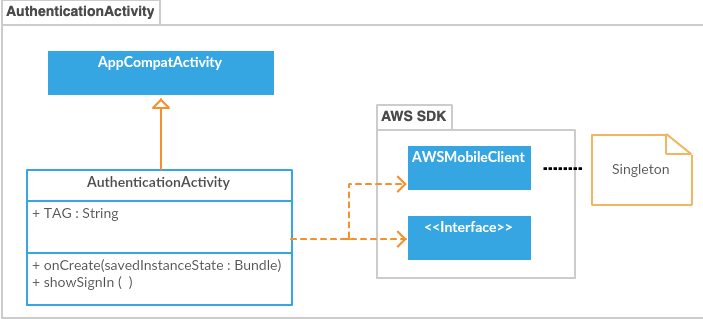
\includegraphics[width=0.9\textwidth, keepaspectratio]{../includes/pics/authenticationactivity.png}
            \caption{Diagramma della classe AutenticationActivity}
        \end{center}
        \end{figure}


   \item \emph{MainActivity}: è la schemata principale che mostra la lista di Workflow dell'utente;
        \begin{figure}[H]
	    \begin{center}
		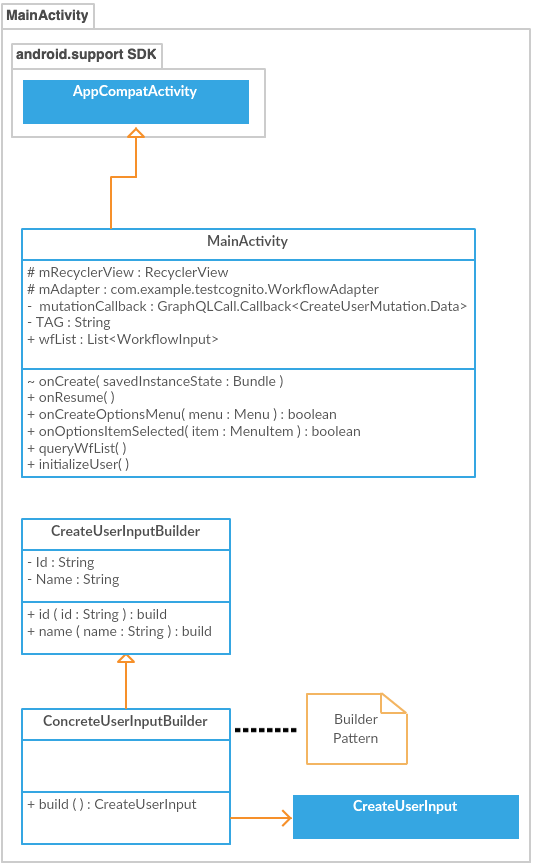
\includegraphics[width=0.8\textwidth, keepaspectratio]{../includes/pics/mainactivity.png}
		\caption{Diagramma della classe MainActivity}
	    \end{center}
        \end{figure}
        

    \item \emph{AddWorkflowActivity}: è l'activity che consente di inserire un nuovo workflow;
       \begin{figure}[H]
	   \begin{center}
    
		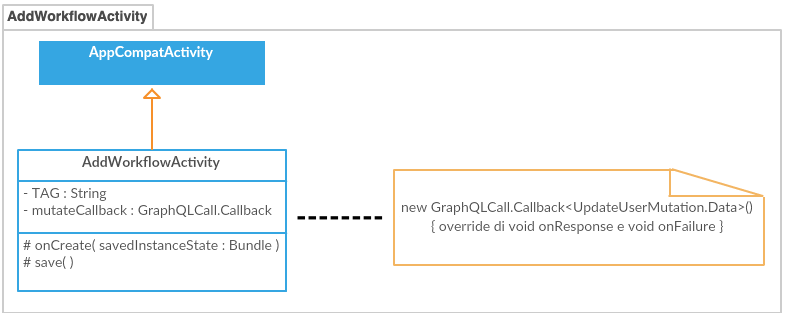
\includegraphics[width=0.9\textwidth, keepaspectratio]{../includes/pics/addworkflowactivity.png}
		\caption{Diagramma della classe AddWorkflowActivity}
	   \end{center}
       \end{figure}
   
   
   
    \item \emph{ConnectorActivity}: è l'activity che consente di gestire i connettori relativi al workflow su cui si sta operando;
        \begin{figure}[H]
	    \begin{center}
		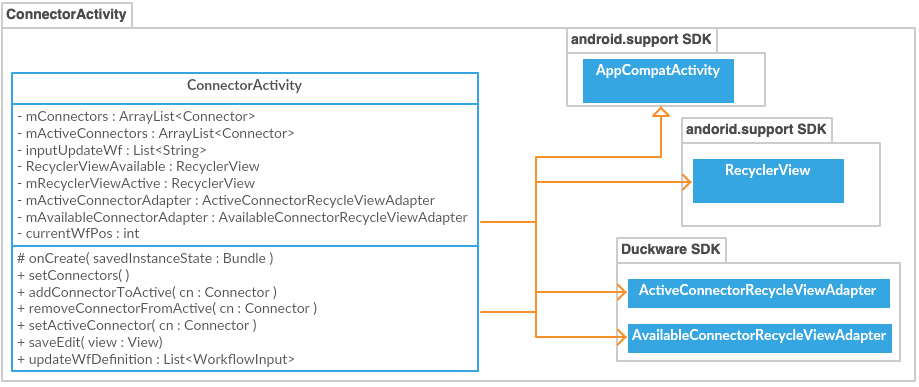
\includegraphics[width=0.9\textwidth, keepaspectratio]{../includes/pics/connectoractivity.png}
		\caption{Diagramma della classe ConnectorActivity}
	    \end{center}
        \end{figure}
    
    
     \item \emph{SetConnectorActivity}: è l'activity che consente di gestire i parametri relativi al connettore su cui si sta operando;
        \begin{figure}[H]
	    \begin{center}
		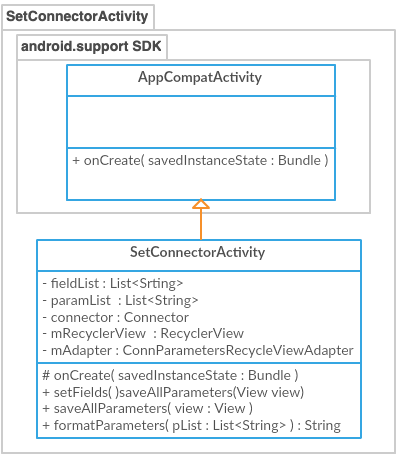
\includegraphics[width=0.9\textwidth, keepaspectratio]{../includes/pics/setconnectoractivity.png}
		\caption{Diagramma della classe SetConnectorActivity}
	    \end{center}
        \end{figure}   
\end{itemize}

È inoltre presente la classe di supporto Connector.java non generata automaticamente da Amplify:
        \begin{figure}[H]
	    \begin{center}
		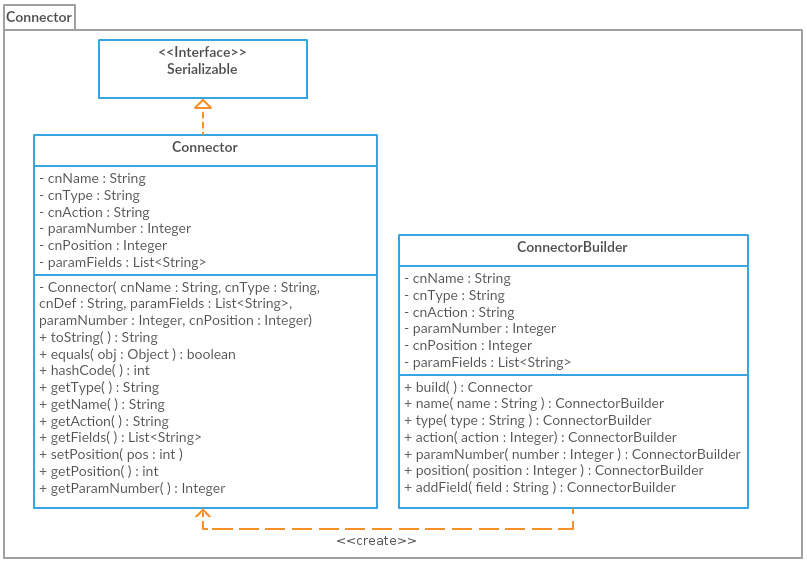
\includegraphics[width=0.75\textwidth, keepaspectratio]{../includes/pics/connector.png}
		\caption{Diagramma della classe Connector}
	    \end{center}
        \end{figure}
        
Questa utilizza un builder pattern poichè i connettori vengono istanziati con attributi eterogenei e a volte vuoti.        

Ogni Activity potrà comunicare con le API solamente utilizzando il client generato dalla classe \emph{ClientFactory}.\\[0.25cm]

\begin{figure}[H]
	\begin{center}
		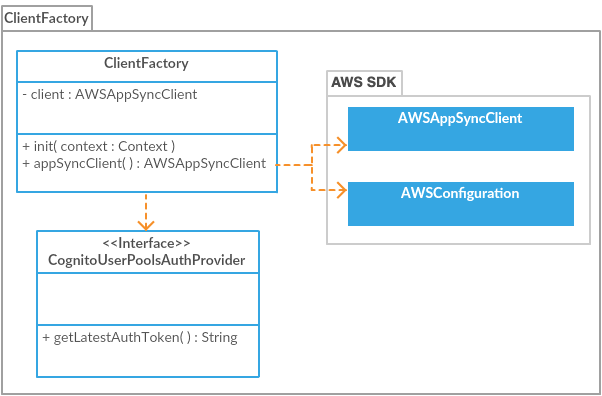
\includegraphics[width=0.9\textwidth, keepaspectratio]{../includes/pics/clientfactory.png}
		\caption{Classe ClientFactory}
	\end{center}
\end{figure}

Le risorse dellínterfaccia grafica sono definite nel namespace res e comprendono i file in linguaggio xml che descrivono gli elementi delle view (layout) e i valori importati da questi elementi (values) quali: 
\begin{itemize}
\item colori;
\item dimensioni;
\item stili;
\item stringhe per lingua italiana;
\item stringhe per lingua inglese;
\end{itemize}



Oltre alle activity e alle risorse xml , è importante notare che tutto il codice necessario alle operazioni sulle risorse backend è definito nel namespace generatedJava, tutto il codice contenuto in questo namespace è generato in automatico da Amplify.

\subsection{Amplify}

Amplify è il framework di Amazon utilizzato per generare un SDK che permette la comunicazione dell'applicazione Android con i servizi in cloud di AWS. La CLI di Amplify consente di sincronizzare i servizi online con l'applicazione, generare librerie di supporto e fornire strumenti di test allo sviluppatore.

\begin{figure}[H]
	\begin{center}
		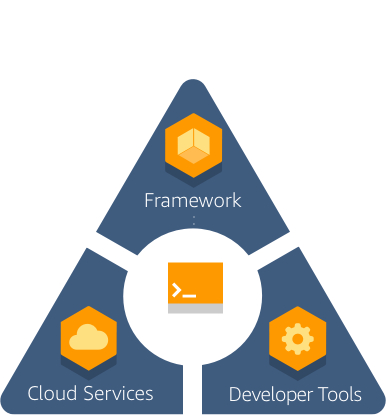
\includegraphics[width=0.55\textwidth, keepaspectratio]{../includes/pics/amplify.png}
		\caption{AWS Amplify}
	\end{center}
\end{figure}

L'integrazione di Amplify in Android Studio consente di delegare controllo e creazione del backend dell'applicazione, noi abbiamo utilizzato Amplify principalmente per due funzioni:

\begin{itemize}
    \item aggiunta di AWS Cognito.
    \item aggiunta di API GraphQL.
\end{itemize}

I metodi per interfacciarsi con Cognito vengono forniti da una libreria di Amazon mentre i metodi per fare query e mutazioni all'endpoint GraphQL vengono generati da Amplify.


Questo è un esempio di query per inserire dati relativi ad un utente:

\begin{verbatim}
     CreateUserInput input = CreateUserInput.builder()
                  .id(AWSMobileClient.getInstance().getUsername())
                  .name(AWSMobileClient.getInstance().getTokens()
                  		.getIdToken().getClaim("nickname"))
                  .build();

        CreateUserMutation addUserMutation = CreateUserMutation.builder()
                .input(input)
                .build();
        com.example.swetlapp.ClientFactory.appSyncClient()
        			.mutate(addUserMutation).enqueue(callback);
\end{verbatim}

CreateUserInput e CreateUserMutation sono due classi generate da Amplify, entrambe sono costruibili tramite builder pattern, AWSMobileClient (singleton) ci permette di comunicare con la user pool di AWS Cognito e ci ritorna informazioni relative all'utente. Quindi si crea l'input per la mutazione, si crea la mutazione stessa, infine esegue questa utilizzando come oggetto di invocazione l'istanza di ClientFactory ritornata dal metodo appSyncClient().\\
Lo schema generale per "comunicare" con le risorse è sempre questo (a meno di query di sola lettura in cui non è necessario costruire un input).


\subsection{Generazione API}

Le API nel nostro caso corrispondono a una soluzione per richieste HTTP ad un endpoint GraphQL.
Per creare e accedere alle API è necessario il servizio AWS AppSync, anche questo sarà settato da amplify.
Componenti principali di AppSync sono:
\begin{itemize}
\item un proxy GraphQl che processa le richieste e le mappa su funzioni e trigger;
\item operazioni: query e mutazioni;
\item data source: nel nostro caso DynamoDB;
\item resolver: converte operazioni GraphQL per essere eseguite sul data source effettivo;
\item AppSync client: dove sono definite le operazioni GraphQL;
\end{itemize}

L'ordine degli eventi per l'impostazione del backend è questo:

\begin{itemize}
\item settaggio di un endpoint GraphQL tramite CLI Amplify;
\item scrittura dello schema delle risorse in linguaggio GraphQL Schema;
\item pubblicazione dello schema;
\item generazione delle API su AppSync (automatico)
\item generazione del database DynamoDB (automatico)
\item generazione dell'SDK per effettuare operazioni definite dallo schema GraphQL (automatico)
\end{itemize}

Lo schema GraphQL che abbiamo scritto è il seguente:
\begin{verbatim}
type User @model {
  id: ID!
  name: String!
  workflow: [Workflow!]
}

type Workflow {
  idwf: ID!
  name: String
  def: String
}
\end{verbatim}


A partire da questo, in dynamoDB è stata generata una tabella User con i campi:
\begin{itemize}
\item id;
\item name;
\item lista di workflow;
\end{itemize}

Amplify genera solo le classi java dei tipi con direttiva \textit{@model}, quindi abbiamo a disposizione solo operazioni con il tipo User, per accedere ai workflow, ai connettori dei workflow e ai parametri dei connettori è necessario operare con il file Json definito dalla stringa \textit{def}, per operare agevolmente con i file Json in ambiente Android abbiamo importato le librerie \textit{import org.json.JSONException} e \textit{import org.json.JSONObject}.

Esempio: per generare il Json nella forma:

\begin{verbatim}
{\"action\":\"connector_action\",\"params\":[\"first_param\",\"second_param\"]}
\end{verbatim}

il codice Java sarà:

\begin{verbatim}
            Map<String, Object> connMap = new HashMap<>();
            connMap.put("action",connector.getAction());
            connMap.put("params",pList);
            JSONObject jsonObject = new JSONObject(connMap);
\end{verbatim}




\pagebreak
\section{Architettura Skill}

L'architettura della skill che risiede in cloud in AWS Lambda è rappresentata dal seguente diagramma:

\begin{figure}[H]
	\begin{center}
		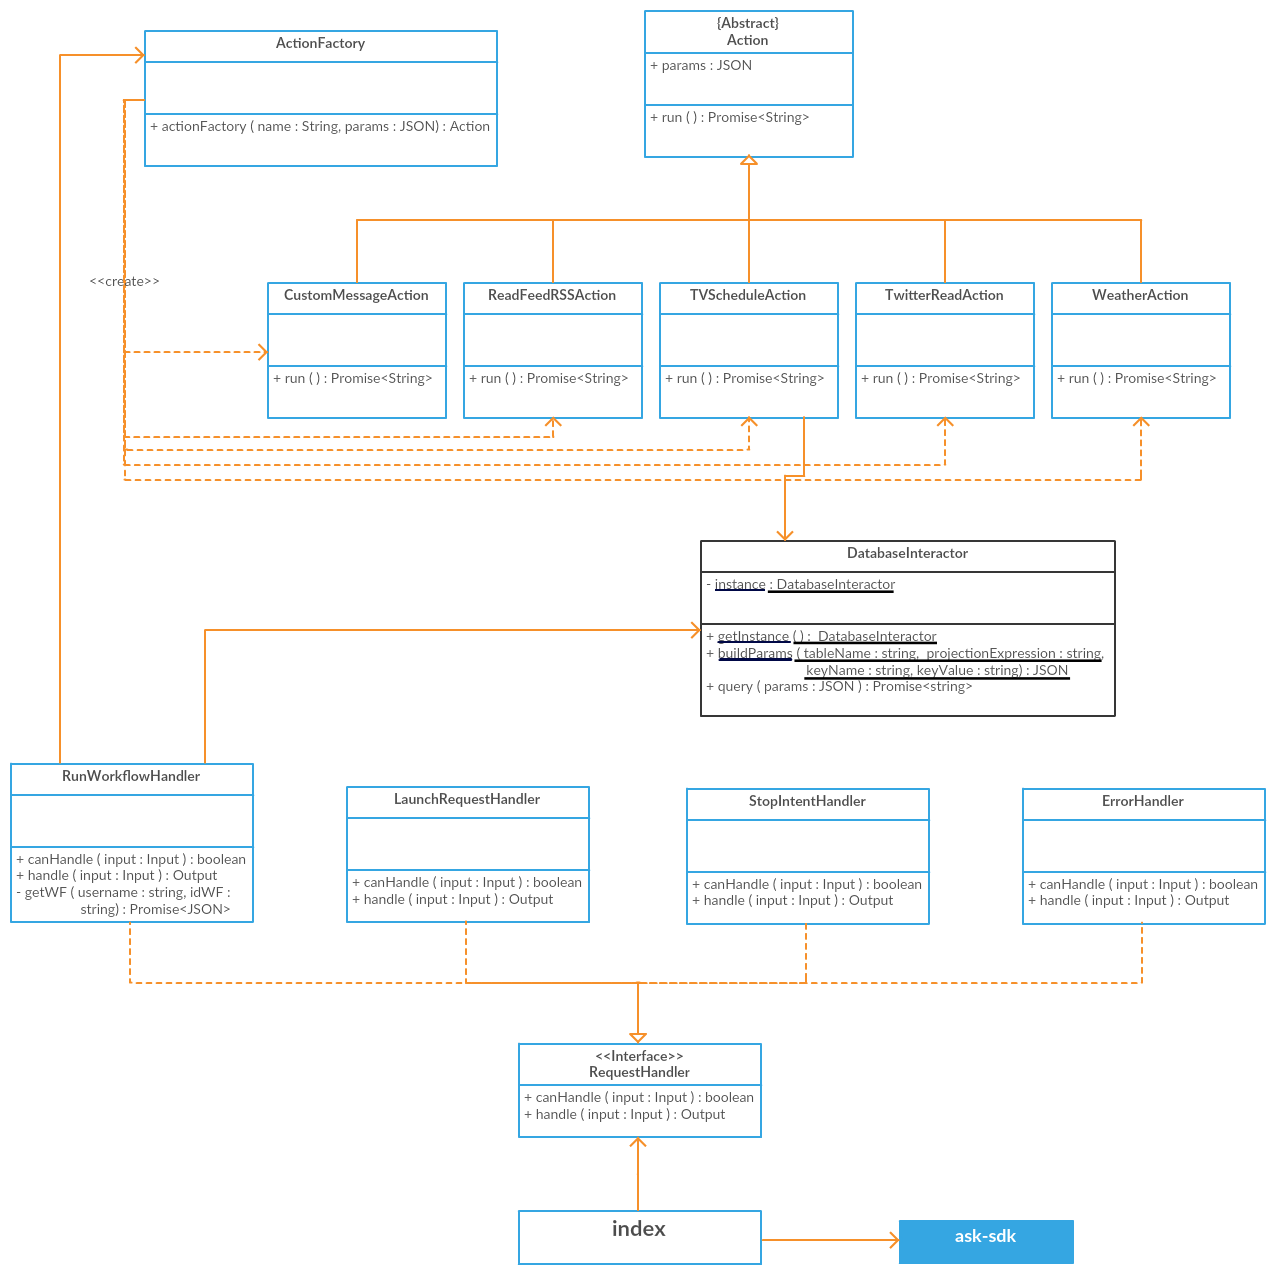
\includegraphics[width=\textwidth, keepaspectratio]{../includes/pics/Skill.png}
		\caption{Overview architetturale della skill.}
	\end{center}
\end{figure}
%TODO descrizione e dire che la struttura generale è visibile nella figura, aggiungere quindi il diagramma della skill completa

\subsection{Back-end}
La logica della skill è gestita dal file index.js al quale Alexa si appoggerà per l'invio delle richieste derivanti dall'interazione con l'utente.
Ogni richiesta inviata incapsula una serie di dati, quali il tipo di \textit{intent} che la attiva e i parametri forniti dall'utente, denominati slot, e sarà gestita da uno degli handler presenti nel file index.js.
Per ognuno di questi verrà eseguito il metodo \textit{canHandle()} e, in caso di ritorno positivo, sarà lanciato il relativo metodo \textit{handle()}, interrompendo la ricerca dell'handler adeguato.
Nel caso in cui non venga trovato alcun gestore appropriato, la skill ha un comportamento non definito che porta al suo arresto improvviso; pertanto la best practice prevede l'implementazione di un handler di default che viene eseguito all'occorrenza di errori.

\subsubsection{Handler}
L'interfaccia RequestHandler è fornita dalle librerie di AWS incluse nel package.
Espone un metodo \textit{canHandle(input : Input)} che ritornerà un booleano: \textit{true} nel caso in cui l'handler che lo ridefinisce dovrà gestire la richiesta passatagli; \textit{false} altrimenti.
Nel caso di ritorno positivo, verrà eseguito il metodo \textit{handle(input : Input)} fornito dall'interfaccia; la sua ridefinizione dovrà elaborare la richiesta in input per poter fornire un ritorno \textit{Output} comprensibile da Alexa.
Gli handler sono strutturati con uno strategy pattern descritto nel seguente diagramma:

\begin{figure}[H]
	\begin{center}
		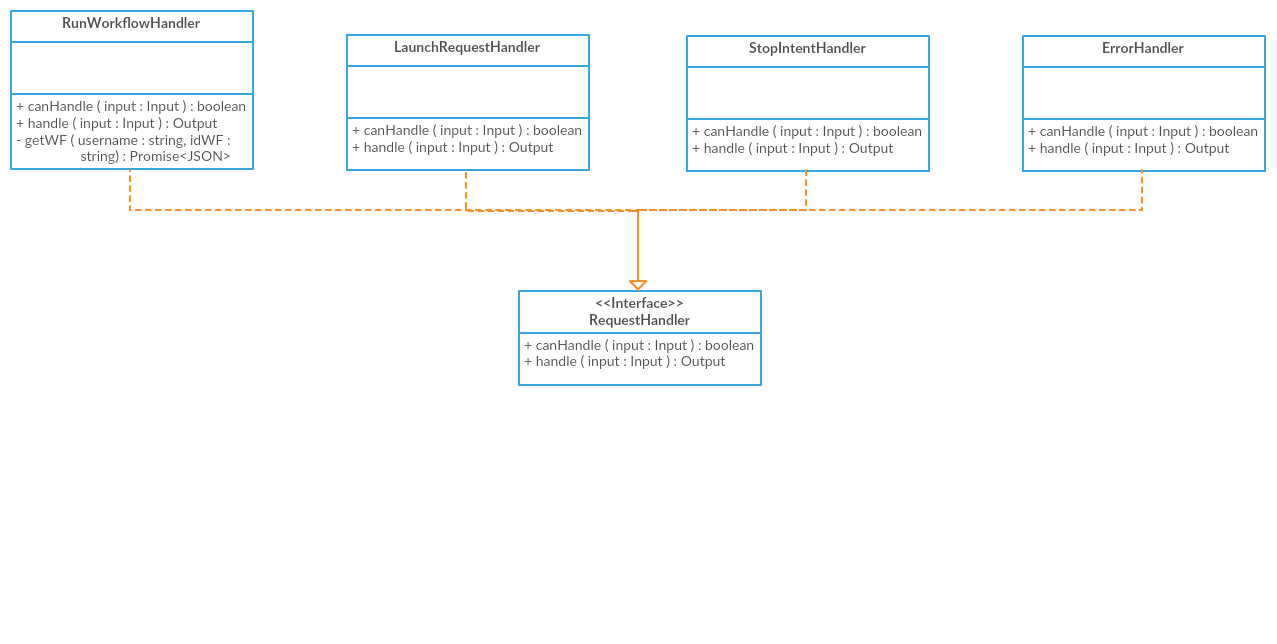
\includegraphics[width=0.9\textwidth, keepaspectratio]{../includes/pics/Strategy Pattern.png}
		\caption{Diagramma della classe Handler}
	\end{center}
\end{figure}


I principali handler da noi definiti sono:
\begin{itemize}
	\item \textit{LaunchRequestHandler}: gestisce il lancio iniziale della skill controllando che l'utente sia autenticato; in caso contrario lo invita ad effettuare il login con una notifica vocale e una push nell'applicazione Amazon Alexa dell'utente;
	\item \textit{RunWorkflowHandler}: viene lanciato quando l'utente richiede l'avvio di un workflow; si occupa di fare una query al database per ottenere i dati del workflow richiesto, quando disponibile, e cominciare la sua esecuzione;
	\item \textit{StopIntentHandler}: elabora la richiesta di arresto della skill da parte dell'utente;
	\item \textit{ErrorHandler}: è il gestore di default che verrà eseguito quando nessuno dei precedenti handler è stato avviato, o nel caso in cui si siano verificati errori durante l'esecuzione della skill;
\end{itemize}

\subsubsection{Action}
I workflow sono composti di azioni;
la loro struttura è definita da Action, questa è una classe astratta ed espone un metodo \textit{run()} che verrà chiamato per l'effettiva esecuzione dell'azione specifica.
La sua ridefinizione delinea il comportamento dell'azione concreta.\\
Le azioni ridefinite nella Skill SwetlApp sono:
\begin{itemize}
	\item \textit{CustomMessageAction}: consente ad Alexa di leggere un messaggio definito dall'utente;
	\item \textit{ReadFeedRSSAction}: consente ad Alexa di ricevere e leggere un feed rss impostato dall'utente;
	\item \textit{TVScheduleAction}: consente ad Alexa di informare l'utente sulla programmazione quotidiana dei suoi canali TV prefereriti;
	\item \textit{TwitterReadAction}: permette ad Alexa di leggere i tweet di un account Twitter definito dall'utente;
	\item \textit{TwitterWriteAction}: permette ad Alexa di postare un tweet personalizzato nella bacheca dell'utente;
\end{itemize}

\subsubsection{ActionFactory}
Si occupa della costruzione di un oggetto concreto di tipo derivante da Action.
Nasconde all'esterno il modo in cui viene scelto quale oggetto costruire, permette di estendere e manutenere velocemente e semplicemente il codice, in quanto per aggiungere una nuova Action sarà sufficiente che questa implementi l'interfaccia, e che venga aggiunto un controllo sul factory perchè questa sia usabile all'esterno.
Il controllo per capire qual è il tipo di azione corretto è fatto a partire dal nome dell'azione che viene chiesto come parametro, su questo sarà svolto uno switch case che ritorna l'azione corretta.

\begin{figure}[H]
	\begin{center}
		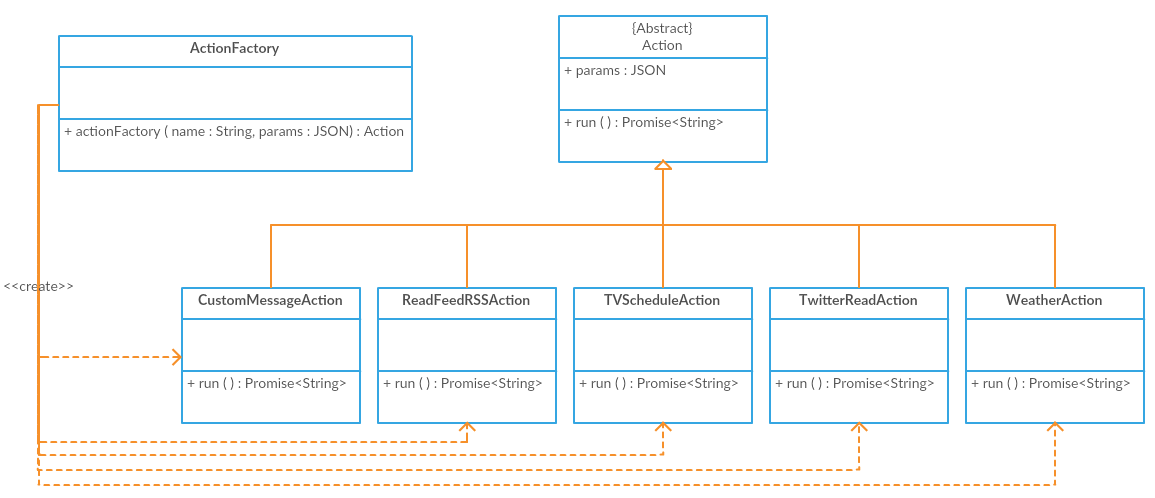
\includegraphics[width=0.9\textwidth, keepaspectratio]{../includes/pics/Factory Pattern.png}
		\caption{Diagramma della classe Action}
	\end{center}
\end{figure}

\subsubsection{Interazione con il database}
La connessione al db è gestita con un pattern singleton che quindi impone l'esistenza di un'unica istanza di \textit{DatabaseInteractor} in un dato momento. L'accesso di più client contemporaneamente al database è possibile perchè AWS si occupa poi di gestire le multiple richieste di accesso al db.
Fornisce un metodo di supporto \textit{query(params : JSON)} per gestire tutte le interazioni con il db direttamente da DatabaseInteractor.


\begin{figure}[H]
	\begin{center}
		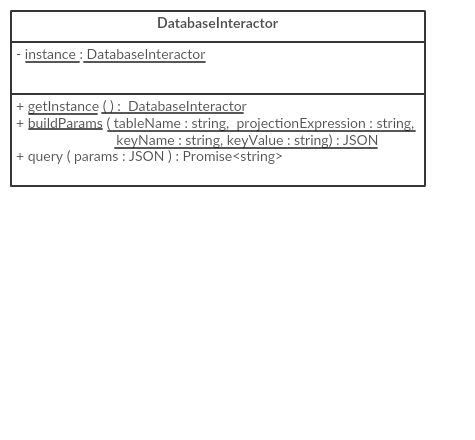
\includegraphics[width=0.75\textwidth, keepaspectratio]{../includes/pics/Singleton Pattern.png}
		\caption{Diagramma della classe DatabaseInteractor}
	\end{center}
\end{figure}

\pagebreak
\section{Licenza}
Copyright 2019 Duckware\\Permission is hereby granted, free of charge, to any person obtaining a copy of this software and associated documentation files (the "Software"), to deal in the Software without restriction, including without limitation the rights to use, copy, modify, merge, publish, distribute, sublicense, and/or sell copies of the Software, and to permit persons to whom the Software is furnished to do so, subject to the following conditions:\\
The above copyright notice and this permission notice shall be included in all copies or substantial portions of the Software.\\
THE SOFTWARE IS PROVIDED "AS IS", WITHOUT WARRANTY OF ANY KIND, EXPRESS OR IMPLIED, INCLUDING BUT NOT LIMITED TO THE WARRANTIES OF MERCHANTABILITY, FITNESS FOR A PARTICULAR PURPOSE AND NONINFRINGEMENT. IN NO EVENT SHALL THE AUTHORS OR COPYRIGHT HOLDERS BE LIABLE FOR ANY CLAIM, DAMAGES OR OTHER LIABILITY, WHETHER IN AN ACTION OF CONTRACT, TORT OR OTHERWISE, ARISING FROM, OUT OF OR IN CONNECTION WITH THE SOFTWARE OR THE USE OR OTHER DEALINGS IN THE SOFTWARE.	
	%%%%%%%%%%%%%%%%%%%%%%%%%%%%%%%%%%%%%%%%%%%%%%%%%%%%%%%%%%%%%%%%%%%%%
\end{document}
